\documentclass[12pt]{letter}

\usepackage{tikz,amsmath,amssymb}
\usetikzlibrary{external,arrows,decorations.pathmorphing,decorations.markings,backgrounds,positioning,fit,petri}
\tikzexternalize

\begin{document}

%bessel function contours
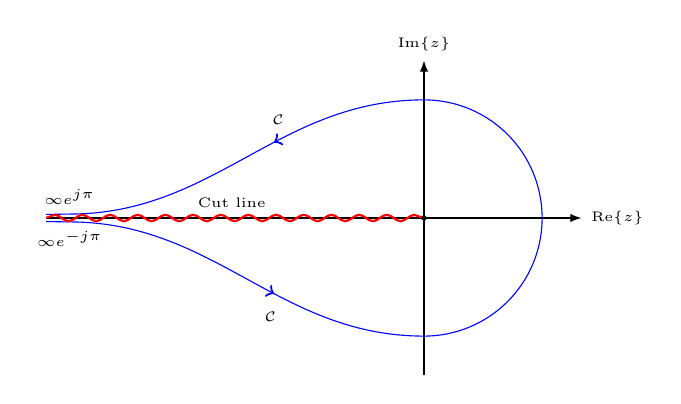
\begin{tikzpicture}
  %draw axes
  \draw [-latex] (-4.8,0) -- (2.0,0) node [right] {\tiny Re$\{z\}$};
  \draw [-latex] (0,-2.0) -- (0, 2.0) node [above] {\tiny Im$\{z\}$};
  %draw upper contour
  \begin{scope}[decoration={markings,
       mark=at position 20mm with {\arrow [blue,thick]{>}}}]
  \draw [blue] (1.5,0) to [out=90,in=0] (0,1.5);
  \draw [postaction={decorate},blue] (0,1.5) to [out=180,in=0] (-4.5, 0.05)
   node [above]{\tiny \textcolor{black}{$\infty e^{j\pi}$}};
  \draw [blue] (-4.8,0.045) -- (-4.5,0.05);
   \node at (-1.85,1.25) {\tiny $\mathcal{C}$};
   \end{scope}
 %draw lower contour
  \begin{scope}[decoration={markings,
       mark=at position 20mm with {\arrowreversed [blue,thick]{>}}}]
  \draw [blue] (1.5,0) to [out=-90,in=0] (0,-1.5);
  \draw [postaction={decorate},blue] (0,-1.5) to [out=180,in=0] (-4.5, -0.05)
   node [below]{\tiny \textcolor{black}{$\infty e^{-j\pi}$}};
  \draw [blue] (-4.8,-0.045) -- (-4.5,-0.05);
  \node at (-1.95,-1.25) {\tiny $\mathcal{C}$};
   \end{scope}
  %draw the cut line
  \draw [red,thick,decorate,decoration={snake,amplitude=0.4mm}] (-4.8,0) -- (0,0)
  node [above,align=center,midway]
  {
  \tiny \textcolor{black}{Cut line}
  };
\fill[black] (0,0) circle (1.0pt);
\end{tikzpicture}


%hankel function contours
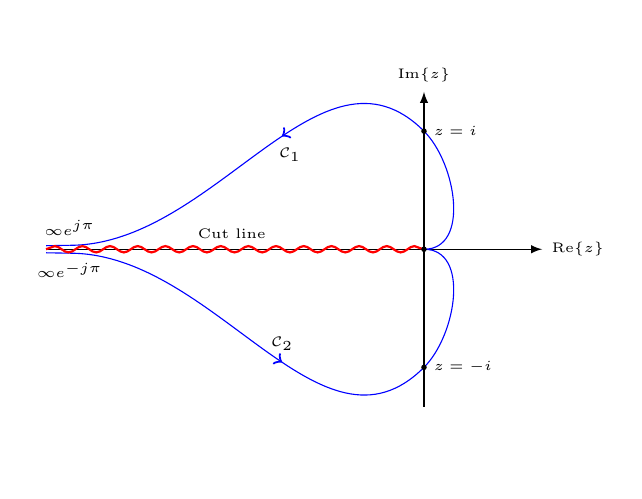
\begin{tikzpicture}
  %draw axes
  \draw [-latex] (-4.8,0) -- (1.5,0) node [right] {\tiny Re$\{z\}$};
  \draw [-latex] (0,-2.0) -- (0, 2.0) node [above] {\tiny Im$\{z\}$};
  %draw upper contour
  \begin{scope}[decoration={markings,
       mark=at position 20mm with {\arrow [blue,thick]{>}}}]
  \draw [blue] (0,0) to [out=0,in=-45] (0,1.5);
  \draw [postaction={decorate},blue] (0,1.5) to [out=135,in=0] (-4.5, 0.05)
   node [above]{\tiny \textcolor{black}{$\infty e^{j\pi}$}};
  \draw [blue] (-4.8,0.045) -- (-4.5,0.05);
  \fill [black] (0,1.5) circle (1.0pt) node [right] {\tiny \textcolor{black}{$z = i$}};
   \node at (-1.7,1.2) {\tiny $\mathcal{C}_1$};
   \end{scope}
  %draw lower contour
   \begin{scope}[decoration={markings,
       mark=at position 20mm with {\arrowreversed [blue,thick]{>}}}]
  \draw [blue] (0,0) to [out=0,in=45] (0,-1.5);
  \draw [postaction={decorate},blue] (0,-1.5) to [out=-135,in=0] (-4.5, -0.05) node [below]{\tiny \textcolor{black}{$\infty e^{-j\pi}$}};
  \draw [blue] (-4.8,-0.045) -- (-4.5,-0.05);
  \fill [black] (0,-1.5) circle (1.0pt) node [right] {\tiny \textcolor{black}{$z = -i$}};
  \node at (-1.8,-1.2) {\tiny $\mathcal{C}_2$};
  \end{scope}
  %draw the cut line
  \draw [red,thick,decorate,decoration={snake,amplitude=0.4mm}] (-4.8,0) -- (0,0)
  node [above,align=center,midway]
  {
  \tiny \textcolor{black}{Cut line}
  };
  \fill[black] (0,0) circle (1.0pt);
\end{tikzpicture}

\end{document}
